

\begin{frame}[fragile]
\frametitle{Erreichtes: Code}


%\only<1>
%	{ 
%\framebox{   %   % just so you can see where the "picture" is

\only<1>
	{
%	\begin{picture}(100,70)
%		\put(15,0){
\begin{center}
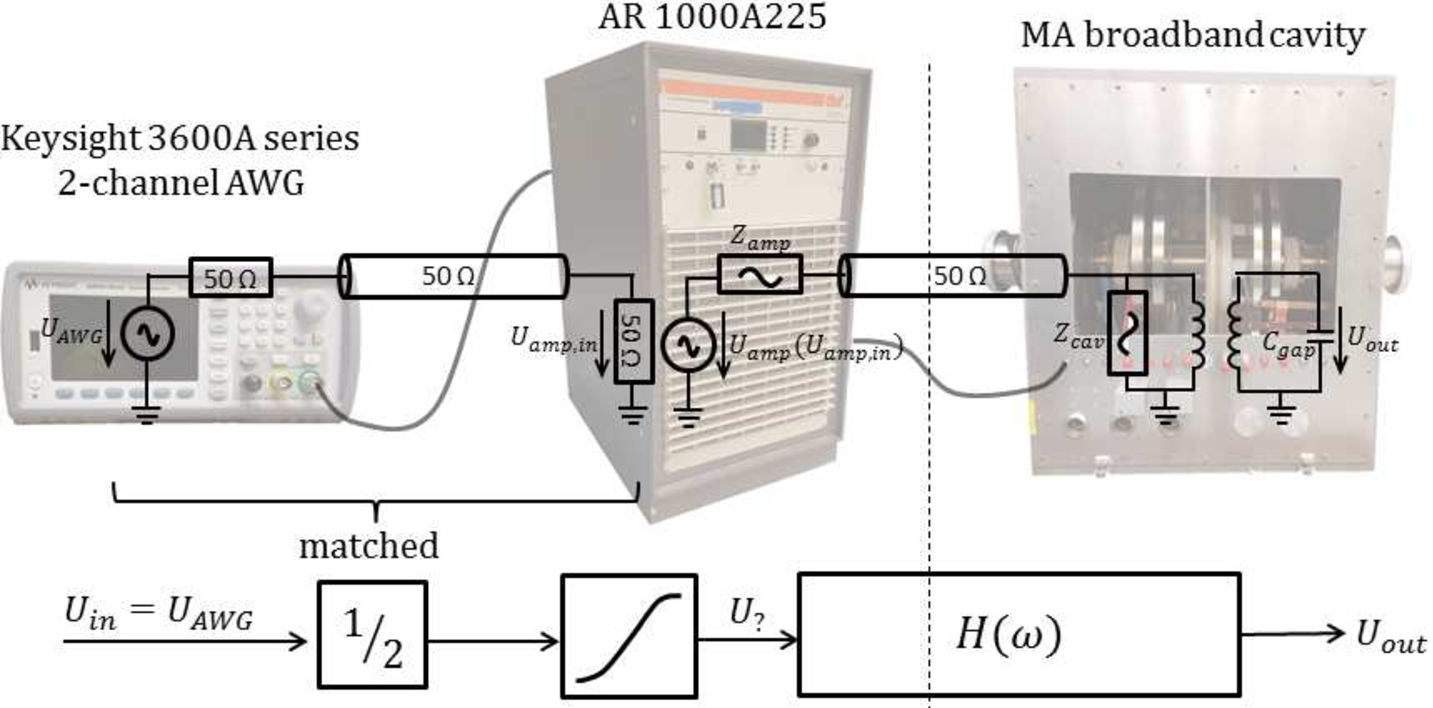
\includegraphics[scale=0.45]{slides/ResultCode/WEPVA047f2_2-eps-converted-to.pdf} 
\end{center}
			
%		}  
%	\end{picture} 
	}

\only<2>
	{
	\begin{picture}(100,70)
		\put(15,0){
			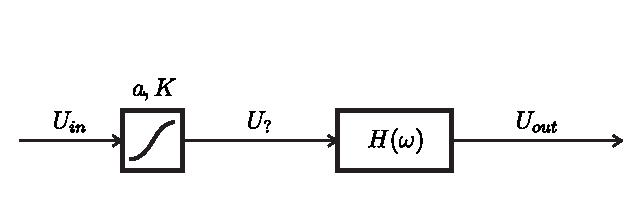
\includegraphics[scale=1.0]{slides/ResultCode/Slide1.eps} 
		}  
	\end{picture} 
	}
		
\only<3>
	{
	\begin{picture}(100,70)
		\put(15,0){
			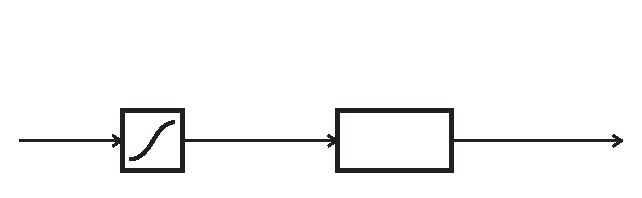
\includegraphics[scale=1.0]{slides/ResultCode/Slide2.eps} 
		}  
	\end{picture} 
	}

\only<4>
	{
	\begin{picture}(100,70)
		\put(15,0){
			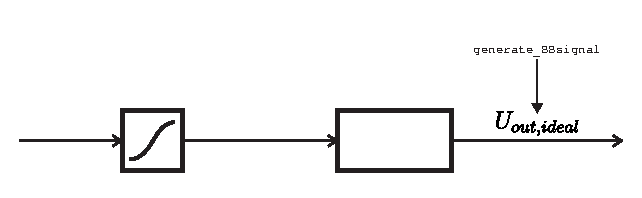
\includegraphics[scale=1.0]{slides/ResultCode/Slide3.eps} 
		}  
	\end{picture} 
	\lstinputlisting[firstline=1,lastline=1]{slides/ResultCode/file.txt} 
	}	

\only<5>
	{
	\begin{picture}(100,70)
		\put(15,0){
			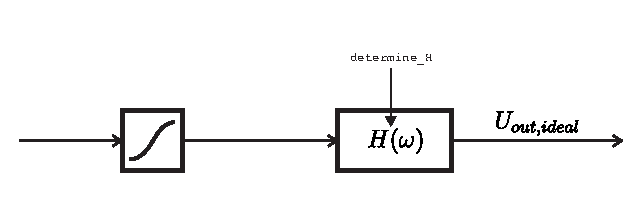
\includegraphics[scale=1.0]{slides/ResultCode/Slide4.eps} 
		}  
	\end{picture} 
	\lstinputlisting[firstline=1,lastline=2]{slides/ResultCode/file.txt} 
	}

\only<6>
	{
	\begin{picture}(100,70)
		\put(15,0){
			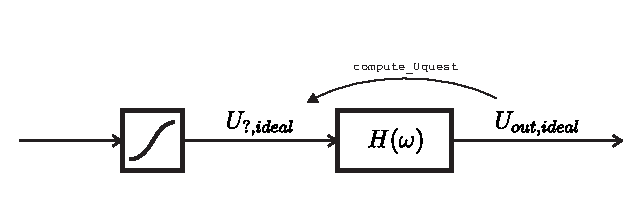
\includegraphics[scale=1.0]{slides/ResultCode/Slide5.eps} 
		}  
	\end{picture} 
	\lstinputlisting[firstline=1,lastline=3]{slides/ResultCode/file.txt} 
	}	
	
\only<7>
	{
	\begin{picture}(100,70)
		\put(15,0){
			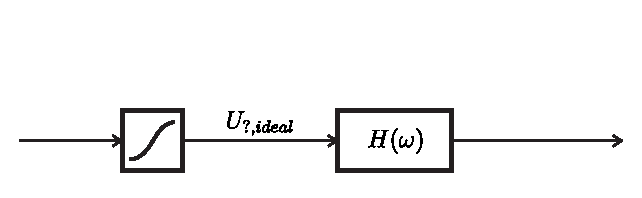
\includegraphics[scale=1.0]{slides/ResultCode/Slide5-1.eps} 
		}  
	\end{picture} 
	\lstinputlisting[firstline=1,lastline=3]{slides/ResultCode/file.txt} 
	}	

\only<8>
{
	\begin{picture}(100,70)
		\put(15,0)
		{
			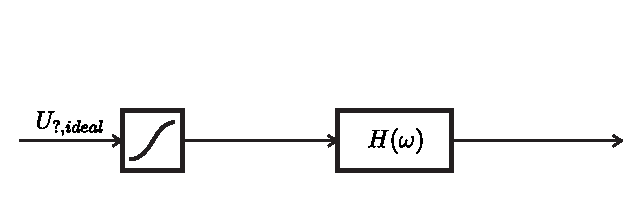
\includegraphics[scale=1.0]{slides/ResultCode/Slide6.eps} 
		}  
	\end{picture} 
	\lstinputlisting[firstline=1,lastline=3]{slides/ResultCode/file.txt} 
}

\only<9>
{
	\begin{picture}(100,70)
		\put(15,0)
		{
			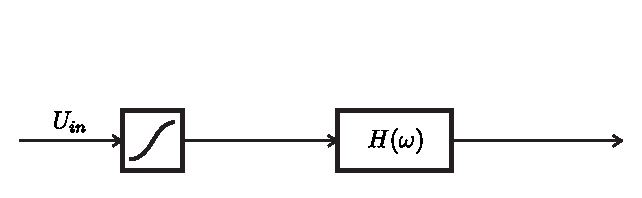
\includegraphics[scale=1.0]{slides/ResultCode/Slide7.eps} 
		}
	\end{picture} 	
	\lstinputlisting[firstline=1,lastline=4]{slides/ResultCode/file.txt} 	
}	
	

\only<10>
{
			\begin{picture}(100,70)
		\put(15,0)
		{
			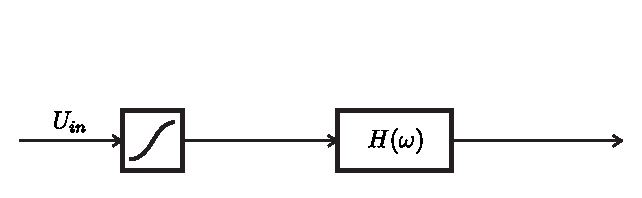
\includegraphics[scale=1.0]{slides/ResultCode/Slide7.eps} 
		}
	\end{picture} 	
	\lstinputlisting[firstline=1,lastline=5]{slides/ResultCode/file.txt} 



\ifnum\WertA=2		
   \begin{textblock}{20}(80,50)
      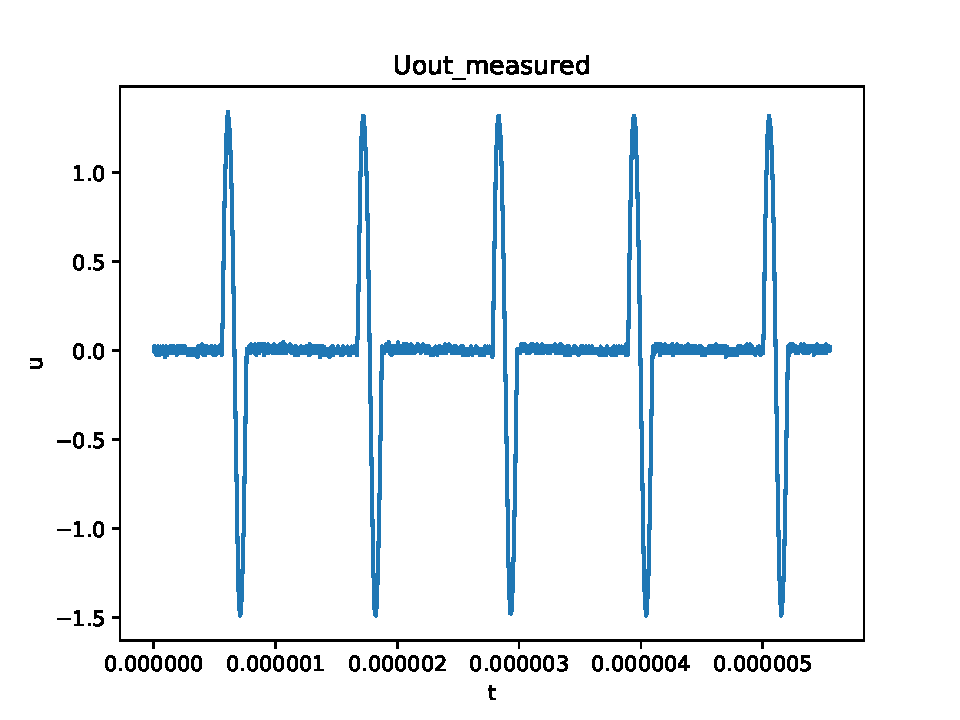
\includegraphics[height=3.5cm, width=4.5cm ]{slides/ResultCode/plots/Uout_1.pdf} 
    \end{textblock}
\fi		
		
%		\begin{picture}(0,20)
%			\put(0,-50)
%			{
%				\framebox(330,20)[]
%				{
%				}			
%			}
%		\end{picture}
%		
%		\begin{picture}(0,0)
%			\put(0,-70)
%			{
%				\framebox(330,20)[]
%				{
%				}			
%			}
%		\end{picture}

%		\begin{picture}(0,0)
%			\put(0,-160)
%			{
%				\framebox(330,50)[]
%				{
%%					\put(-155,100)
%%					{
%%%						\framebox(300,60)[]
%%%						{
%%							\begin{picture}(100,70)
%%							\put(15,0)
%%		{
%%		\begin{figure}
%%		\end{figure}
%%							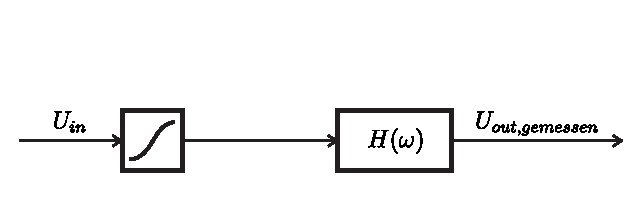
\includegraphics[scale=1.0]{slides/ResultCode/Slide8.eps}
%%							\linebreak
%%							\lstinputlisting[firstline=1,lastline=10]{slides/ResultCode/file.txt}
%%							}
%%							\end{picture} 
%%					%		\lstinputlisting[firstline=1,lastline=10]{slides/ResultCode/file.txt} %
%%%						}					
%%					}				
%%					%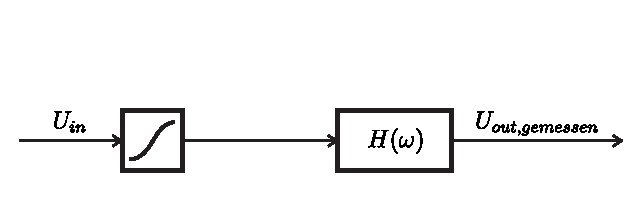
\includegraphics[scale=1.0]{slides/ResultCode/Slide8.eps}
%				}
%%			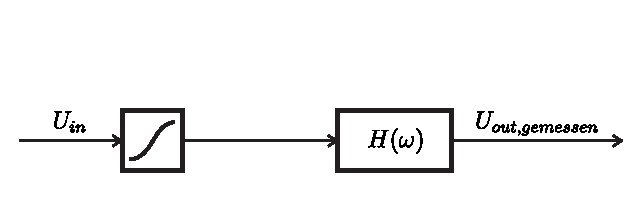
\includegraphics[scale=1.0]{slides/ResultCode/Slide8.eps} %
%			}  
%		\end{picture} 
%		
%		\begin{picture}(0,0)
%			\put(0,-100)
%			{
%				\framebox(330,50)[]
%				{
%				}
%			}  
%		\end{picture} 
%%		\lstinputlisting[firstline=1,lastline=10]{slides/ResultCode/file.txt} %
%	
%	
%%	\begin{picture}(100,100)
%%		\put(10,0)
%%		{
%%			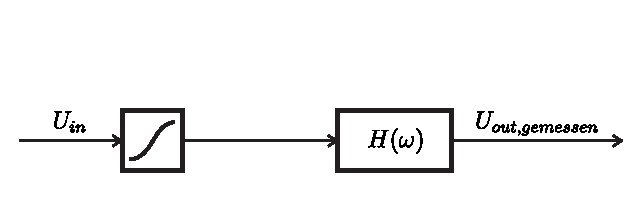
\includegraphics[scale=1.0]{slides/ResultCode/Slide8.eps} 				
%%		}		
%%		\lstinputlisting[firstline=1,lastline=1]{slides/ResultCode/file.txt} 	
%%	\end{picture} 
%%%	\begin{picture}(100,100)
%%%	\begin{picture}(0,0)
%% 		
%%	\end{picture} 
%%	\end{picture} 
%	\begin{picture}(0,0)
% 		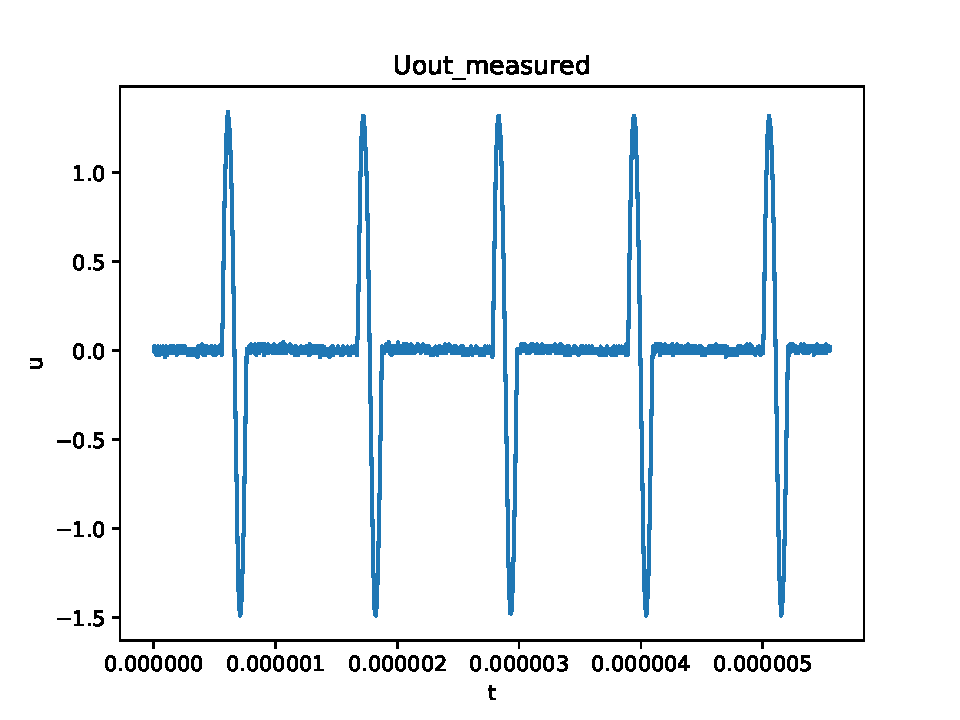
\includegraphics[height=3cm, width=5cm ]{slides/ResultCode/plots/Uout_1.pdf} 
%	\end{picture} 
%
%	 
%%		\put(0,0)
%%		{
%%			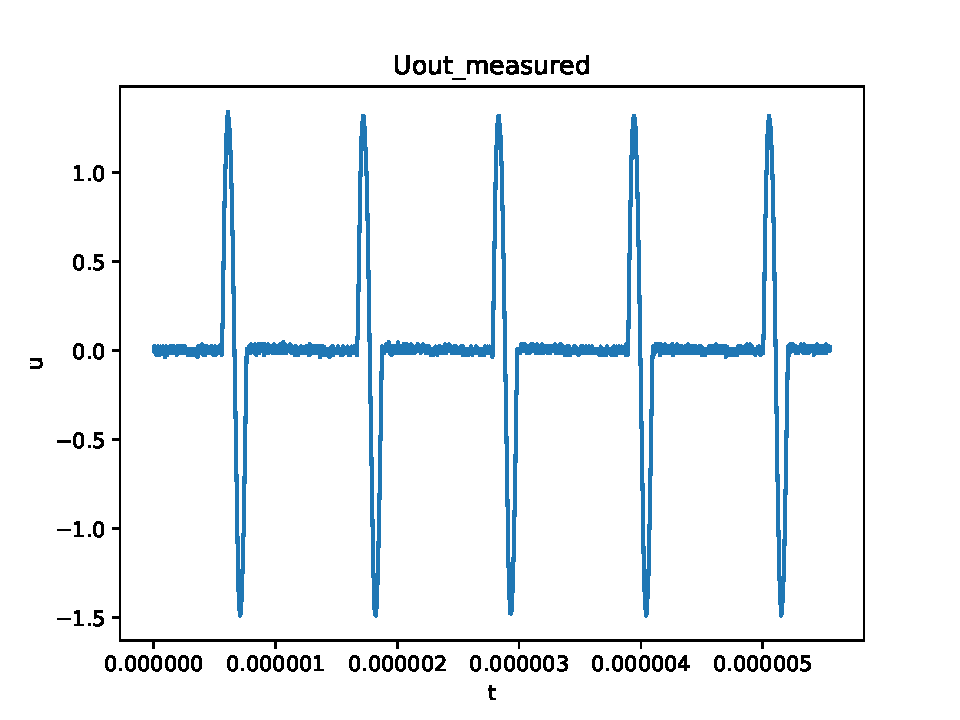
\includegraphics[height=3cm, width=5cm ]{slides/ResultCode/plots/Uout_1.pdf} 
%%		} 
}


\only<11>
	{
	\begin{picture}(100,70)
		\put(15,0){
			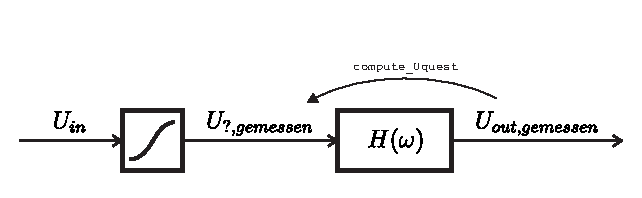
\includegraphics[scale=1.0]{slides/ResultCode/Slide9.eps} 
		}  
	\end{picture} 
	\lstinputlisting[firstline=1,lastline=6]{slides/ResultCode/file.txt} 
	}	
	
\only<12>
	{
	\begin{picture}(100,70)
		\put(15,0){
			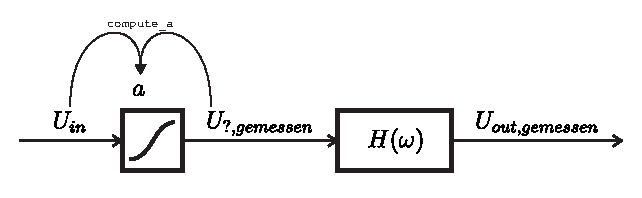
\includegraphics[scale=1.0]{slides/ResultCode/Slide10.eps} 
		}  
	\end{picture} 
	\lstinputlisting[firstline=1,lastline=7]{slides/ResultCode/file.txt} 
	}

\only<13>
	{
	\begin{picture}(100,70)
		\put(15,0){
			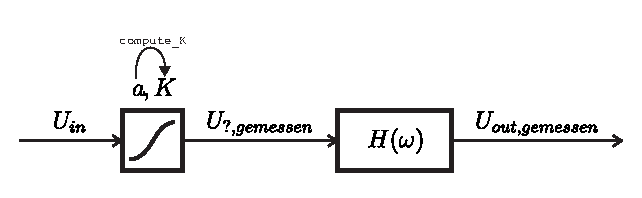
\includegraphics[scale=1.0]{slides/ResultCode/Slide11.eps} 
		}  
	\end{picture} 
	\lstinputlisting[firstline=1,lastline=8]{slides/ResultCode/file.txt} 
	}	

\only<14>
	{
	\begin{picture}(100,70)
		\put(15,0){
			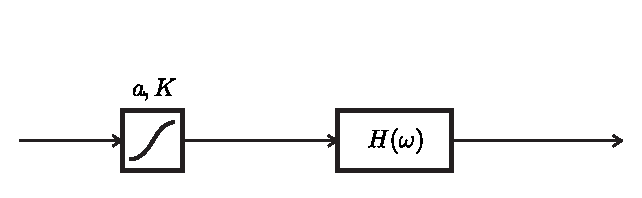
\includegraphics[scale=1.0]{slides/ResultCode/Slide12-0.eps} 
		}  
	\end{picture} 
	\lstinputlisting[firstline=1,lastline=8]{slides/ResultCode/file.txt} 
	}
	
\only<15>
	{
	\begin{picture}(100,70)
		\put(15,0){
			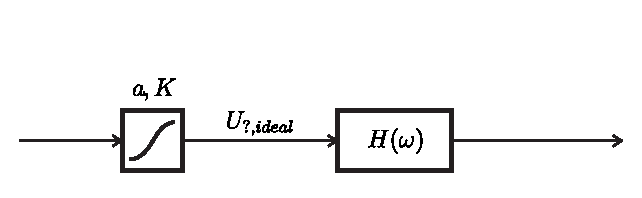
\includegraphics[scale=1.0]{slides/ResultCode/Slide12-01.eps} 
		}  
	\end{picture} 
	\lstinputlisting[firstline=1,lastline=8]{slides/ResultCode/file.txt} 
	}
	
\only<16>
	{
	\begin{picture}(100,70)
		\put(15,0){
			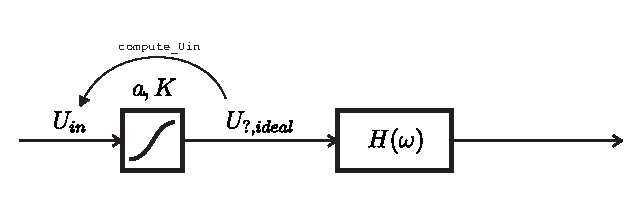
\includegraphics[scale=1.0]{slides/ResultCode/Slide12.eps} 
		}  
	\end{picture} 
	\lstinputlisting[firstline=1,lastline=9]{slides/ResultCode/file.txt} 
	}
	
\only<17>
	{
	\begin{picture}(100,70)
		\put(15,0){
			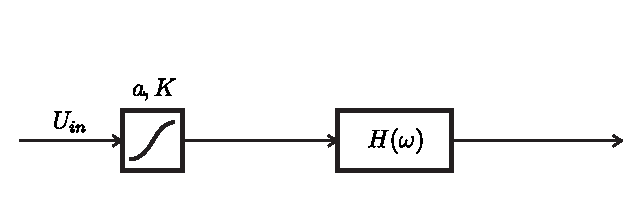
\includegraphics[scale=1.0]{slides/ResultCode/Slide13-0.eps} 
		}  
	\end{picture} 
	\lstinputlisting[firstline=1,lastline=9]{slides/ResultCode/file.txt} 
	}
	
\only<18>
	{
	\begin{picture}(100,70)
		\put(15,0){
			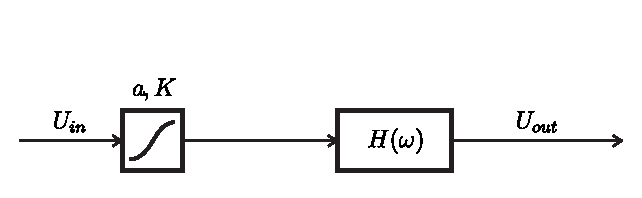
\includegraphics[scale=1.0]{slides/ResultCode/Slide13.eps} 
		}  
	\end{picture} 
	\lstinputlisting[firstline=1,lastline=10]{slides/ResultCode/file.txt} 
	}

  
%	\begin{figure}[t]
%	
%%	
%	\end{figure}	
	%}
%\only<2>{ \lstinputlisting[firstline=1,lastline=2]{slides/ResultCode/file.txt} }
%\only<3>{ \lstinputlisting[firstline=1,lastline=3]{slides/ResultCode/file.txt} }
%\only<4>{ \lstinputlisting[firstline=1,lastline=4]{slides/ResultCode/file.txt} }
%\only<5>{ \lstinputlisting[firstline=1,lastline=5]{slides/ResultCode/file.txt} }
%\only<6>{ \lstinputlisting[firstline=1,lastline=6]{slides/ResultCode/file.txt} }
%\only<7>{ \lstinputlisting[firstline=1,lastline=7]{slides/ResultCode/file.txt} }
%\only<8>{ \lstinputlisting[firstline=1,lastline=8]{slides/ResultCode/file.txt} }
%\only<9>{ \lstinputlisting[firstline=1,lastline=9]{slides/ResultCode/file.txt} }
%\only<10>{ \lstinputlisting[firstline=1,lastline=10]{slides/ResultCode/file.txt} }


\end{frame}



